
\hwpart{III}{Help Your ``Classmate'' Debug (15 points)}
Your classmate Kale is having some trouble getting her model to work. As someone who has successfully trained a DDPM model, you decide to help!

In each of the following scenario, you may be provided a loss curve, a grid of samples or a description of the situation. Try your best to help Kale with her implementation!

\question{Pseudo Debugging Scenarios}{15}

\subq{a}{5} Kale trained a model for 1000 iterations and observed this seemingly nice looking loss curve. However, all her samples are pure noise. What could be the problem here? List at least two potential sources of bugs.
\hwimagepair{q5a_loss_curve.png}{q5a_samples.png}{The loss curve she observed}{The final samples she obtained}{The loss curve and the samples that Kale observed.}

\answerbox{}{
A decreasing training loss does not guarantee that the sampling code is
correct. During training, the model is only optimized to predict the Gaussian
noise \(\epsilon\) from \(x_t\) and \(t\):
\[
\mathcal{L}
=
\mathbb{E}_{x_0,t,\epsilon}
\left[
\|\epsilon - \epsilon_\theta(x_t,t)\|^2
\right].
\]
Thus, Kale's loss curve can look reasonable even if the reverse sampling path is
broken.

One likely bug is an incorrect reverse-process formula. In DDPM sampling, the
predicted noise should be used to compute
\[
\mu_\theta(x_t,t)
=
\frac{1}{\sqrt{\alpha_t}}
\left(
x_t -
\frac{\beta_t}{\sqrt{1-\bar{\alpha}_t}}
\epsilon_\theta(x_t,t)
\right).
\]
If the sign, coefficient, posterior variance, or timestep indexing is wrong,
the sampler may fail to remove noise even though the training MSE decreases.

Another likely bug is incorrect timestep handling in the sampling loop. Sampling
should start from \(x_T \sim \mathcal{N}(0,I)\) and iterate backward from
\(T-1\) to \(0\). If the loop runs in the wrong direction, has an off-by-one
error, or passes the wrong timestep tensor to the model, the U-Net will denoise
under a noise level different from what it saw during training.

I would also check whether the training and sampling schedules match exactly,
including \(\beta_t\), \(\alpha_t\), \(\bar{\alpha}_t\), and the number of
timesteps. A mismatch means timestep \(t\) has different meanings during
training and sampling. Finally, Kale should verify that the sampling script
loads the correct trained checkpoint and applies EMA weights if those were used
for evaluation. Although 1000 iterations may be too short for high-quality face
generation, completely pure-noise samples strongly suggest a sampling, schedule,
timestep, or checkpoint-loading bug.
}
\includeanswer{q5a}

\subq{b}{5} Kale observed that after a while her loss would stay at a non-zero level, and it is quite ``bumpy'' -- the loss does not decrease monotonically but instead has small fluctuations. Should she be worried about this? Why does this ``bumpiness'' exist? Can training for longer still be valuable for improving the model performance in her case?

\answerbox{}{
She should not be worried just because the loss is non-zero and bumpy. The DDPM
training objective is an expectation over the data, the timestep, and the
sampled Gaussian noise:
\[
\mathcal{L}
=
\mathbb{E}_{x_0,t,\epsilon}
\left[
\|\epsilon - \epsilon_\theta(x_t,t)\|^2
\right].
\]
Each optimization step only estimates this expectation with one minibatch, one
random timestep per image, and one fresh noise tensor. Therefore, the plotted
per-step loss is a noisy stochastic estimate, not the exact full objective. It
is normal for it to fluctuate locally rather than decrease monotonically.

The loss also does not need to converge to zero. The model has finite capacity,
the data distribution is complex, and different timesteps have different
difficulty. Very noisy large-\(t\) examples contain little visible image
structure, while small-\(t\) examples require fine local denoising. Because a
batch mixes images, timesteps, and random noise, the loss can remain at a
positive plateau even when the model is learning useful denoising behavior.

Training longer can still be valuable as long as the loss is not exploding or
becoming NaN and the samples or evaluation metrics continue to improve. Even if
the scalar MSE changes slowly, additional training may improve high-level face
structure, texture details, sample diversity, EMA weights, and KID/FID. Kale
should look at a moving average of the loss together with sample grids and
distribution metrics instead of judging the model from raw per-iteration loss
alone.
}
\includeanswer{q5b}

\subq{c}{5} After the model fully converged, Kale obtained these samples shown below. What is her bug and how to fix it?
\begin{figure}[H]
    \centering
    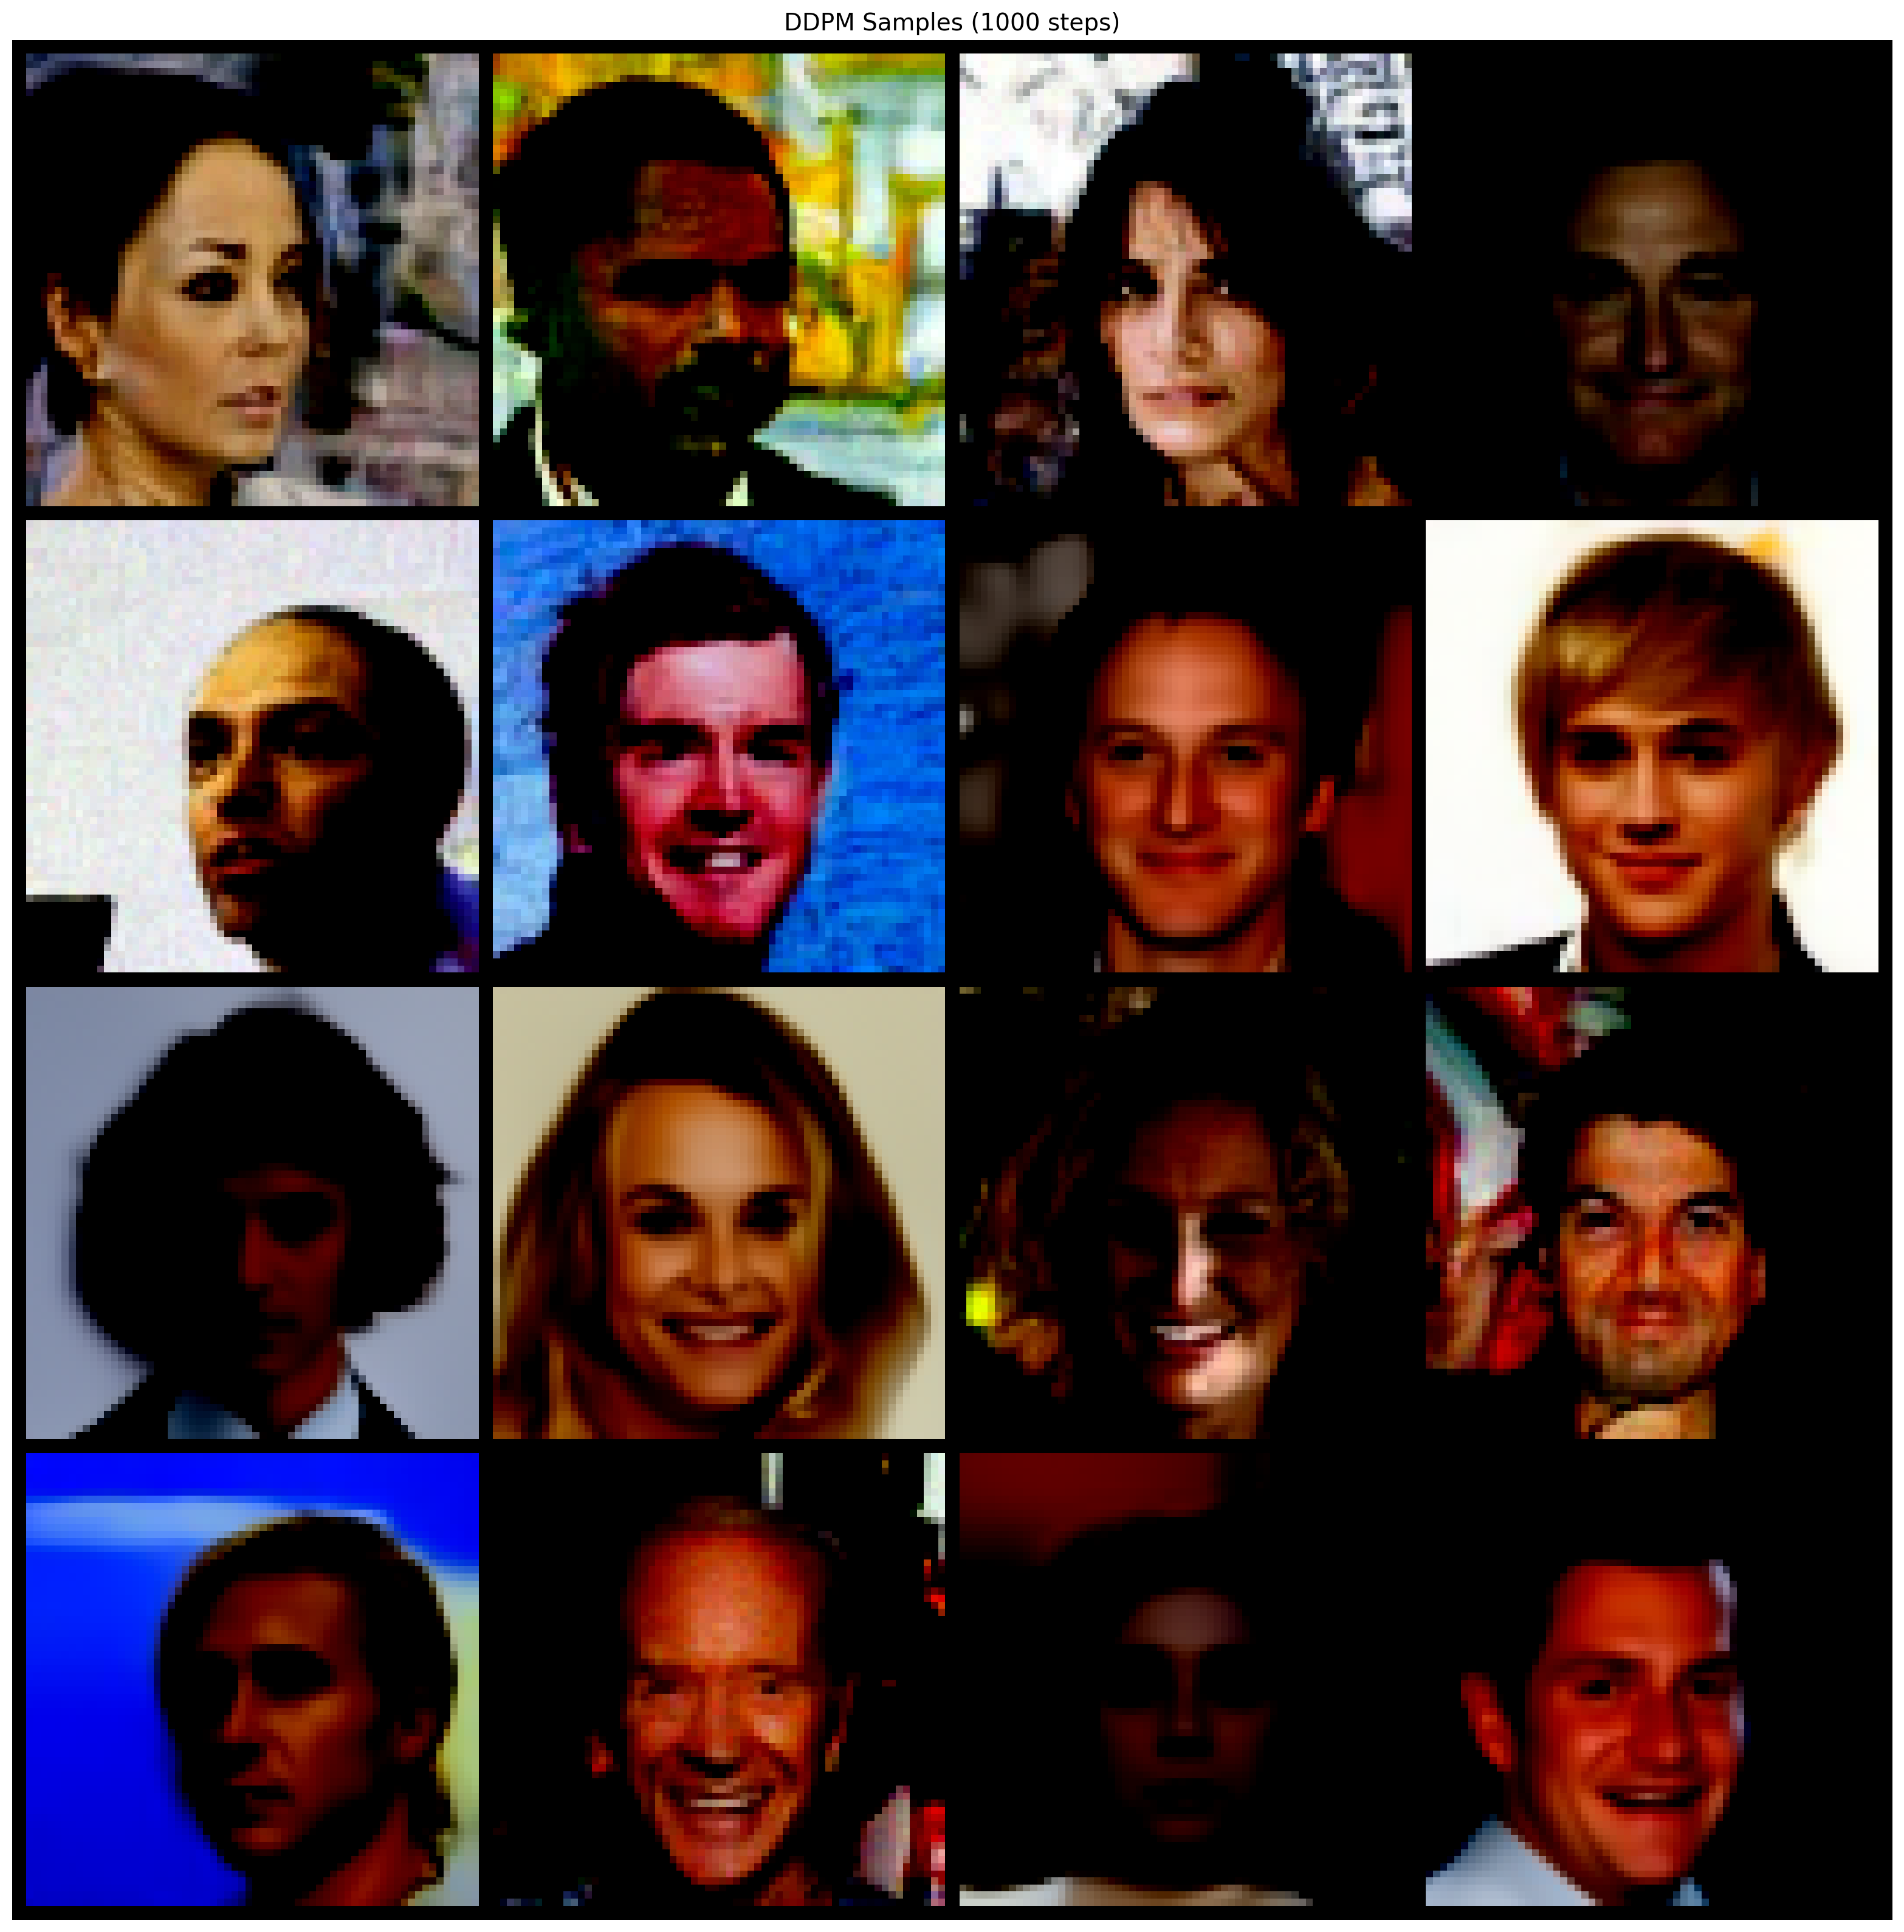
\includegraphics[width=0.5\textwidth]{figures/q5c.png}
    \caption{The samples that Kale obtained.}
\end{figure}

\answerbox{}{
The samples already contain recognizable faces, so the denoising model is not
completely broken. The main issue is that the saved images have an incorrect
value range: large regions are clipped to black and the colors are overly
contrasty. This is the typical symptom of saving tensors from the training
range \([-1,1]\) as if they were display images in \([0,1]\).

Since the training images are normalized before entering the DDPM, the generated
samples should be unnormalized before visualization:
\[
x_{\mathrm{display}}
=
\frac{x_{\mathrm{sample}} + 1}{2},
\qquad
x_{\mathrm{display}}
=
\mathrm{clip}(x_{\mathrm{display}}, 0, 1).
\]
If Kale skips this conversion, all negative pixel values are clipped to zero by
the image-saving pipeline, which explains the dark backgrounds and saturated
appearance.

The fix is to apply the inverse normalization before saving or displaying
samples, for example \texttt{images = ((samples + 1) / 2).clamp(0, 1)}, or to
use a helper such as \texttt{unnormalize(samples).clamp(0, 1)}. She should check
the visualization code before retraining, because this bug can make a
successfully trained model look much worse than it actually is.
}
\includeanswer{q5c}
